% vim: set tw=78 tabstop=4 shiftwidth=4 aw ai:

\chapter{Measurements of Multimedia Distribution in Peer-to-Peer Networks}
\label{chapter:multimedia-dist}

A large part of content distribution in the Internet is currently video
content. Video content means large files, typically movie files of CD or DVD
size. File size increases if the bitrate or resolution increases. Apart from
movie files, sites such as YouTube, focusing on small videos that are
published by average users are attracting millions of users. Content is
accessed many times and transferred across the Internet.

A Peer-to-Peer protocol and BitTorrent, in particular, is one of the most
adequate solution for distributing large content. Rapid creation of swarms,
tit-for-tat, rarest-piece first allow BitTorrent to rapidly distributed files
among peers. When thinking about video content, this mode is known as offline
playback -- the video file is downloaded and subsequently rendered. Separate
approaches are to be undertaken for Video-on-Demand and Live Streaming as
described in Section~\ref{sec:multimedia-dist:video}.

\section{Adding Video Streaming Support in libtorrent}
\label{sec:multimedia-dist:libtorrent}

libtorrent-rasterbar\footnote{\url{http://www.rasterbar.com/products/libtorrent/}}
is a popular solution implementing the BitTorrent
specification\footnote{\url{http://bittorrent.org/beps/bep\_0003.html}} and many of
its enhancements.  Written in C++ it uses advanced operating system operations
allowing good performance. It is used by a large number of BitTorrent clients,
including Deluge, Miro, qBitTorrent, ZipTorrent, LimeWire.

As, from a performance point of view, libtorrent-rasterbar possesses a high
rank among BitTorrent implementations, it was considered as one of the best
choices for adding streaming support. libtorrent-rasterbar is used only
as a classical BitTorrent distribution solution, not as a streaming solution.
The goal was to provide video on demand (VoD) support by altering the required
components of the implementation.

The piece selection strategy in a typical BitTorrent swarm is based on
\textit{rarest-first}. This means that each peer tries to acquire the rarest
piece as the first one ensuring better performance that random packet
selection~\cite{bt-analysis}\cite{scaling-networks}. An analysis has proven that
\textit{rarest-first} has the best performance when considering the efficiency
vs. cost factor.

As a consequence of the particularities of the ``strictly in order'' piece
selection algorithm, \textit{tit-for-tat} can not be used within a single
swarm. Peer relations are asymmetrical and a downloader may never serve
pieces to an uploader. This means that piece requests are non-uniformly
distributed among the whole swarm. Old peers receive more requests that
younger peers but may only serve \textbf{U} of them.

Presuming, as it usually is the case, a connection that possesses a bandwidth
capacity higher than the playback rate, an efficient streaming doesn't need to
employ \textit{strictly in order} piece selection. It only needs a sufficient
number of packages that allow content playback to happen at a consistent rate,
while other pieces may be retrieved using other algorithms. A compromise needs
to be negotiated between sequential progress and download speed, download
latency and swarm health.

In order to achieve that compromise, we define \textit{deadline pieces}. This
pieces use a deadline specifying when the packet needs to be downloaded. Such
a packet receives a priority in the pieces selection if it's close to its
deadline. This way, some of the packets may be downloaded through
\textit{rarest-first} while others may be downloaded through \textit{strictly
in order}. Deadlines may be computed by taking into account the media bitrate
and the number of pieces of the video asset.

The module implementing the piece selection is a central component in a
BitTorrent implementation. It is optimized in libtorrent to rapidly find
rarest pieces. It keeps a list of available pieces, sorted by rarity, and
equally rare packets are mixed. The \textit{rarest-first} model is the main
strategy for piece selection. Other models are supported, though their use is
particular to certain situations.

The piece selector allows combining the availability of a given packet with a
certain piece priority. These parameters determine the criterion used for
sorting the piece list. Zero priority pieces will never be selected, an option
used for selective downloading.

For \textit{strictly in order} implementation, a specialized option dubbed
\textit{sequential} is added to the piece picker and is checked inside the
\texttt{piece\_picker::pick\_pieces()} function. A \textit{cursor} variable is
inserted that stores the index of the last downloaded piece. The interested
block list is appended the block not already download that can be downloaded
sequentially from the given peer. New blocks are added in the same manner
until the requested block limit is reached or no more pieces are available. To
be remarked that piece request is sequential but not necessarily piece
delivery.

In order to implement the \textit{piece deadline} strategy, a new concept was
added: \textit{time\_critical\_pieces}; these pieces differ from normal pieces
by having a deadline attached (\textit{piece\_deadline}). Within the library,
these pieces are requested in a different manner than normal pieces. Usually,
after a peer completes a request, a new piece request is sent to that peer.
For \textit{deadline} pieces, peer list is searched for peers possessing that
piece. Peers are sorted by download speed and outstanding bytes.

Both for the \textit{piece deadline} strategy and the \textit{strictly
in-order} strategy, there are performance gains if partially available pieces
are prioritized; that is pieces whose block are already available to the peer.
Special thanks go to Arvid Norberg, the main developer behind
libtorrent-rasterbar. He had provided useful tips, suggestions and support
both and the IRC channel and the developer's mailing list.

A sample graph comparing the \textit{rarest first} (blue), \textit{sequential}
(red) and \textit{deadline piece} (yellow) algorithms is shown in
Figure~\ref{fig:multimedia-dist:libtorrent-evolution}. The two
graphs show download evolution (in megabytes) and speed evolution (in KB/s).
The swarm used consisted of several seeders and a high number of leechers.
File size was 37~MB, and the file was spread into 578 pieces.

\begin{figure}
  \centering
  \subfloat[Download Size Evolution]{
  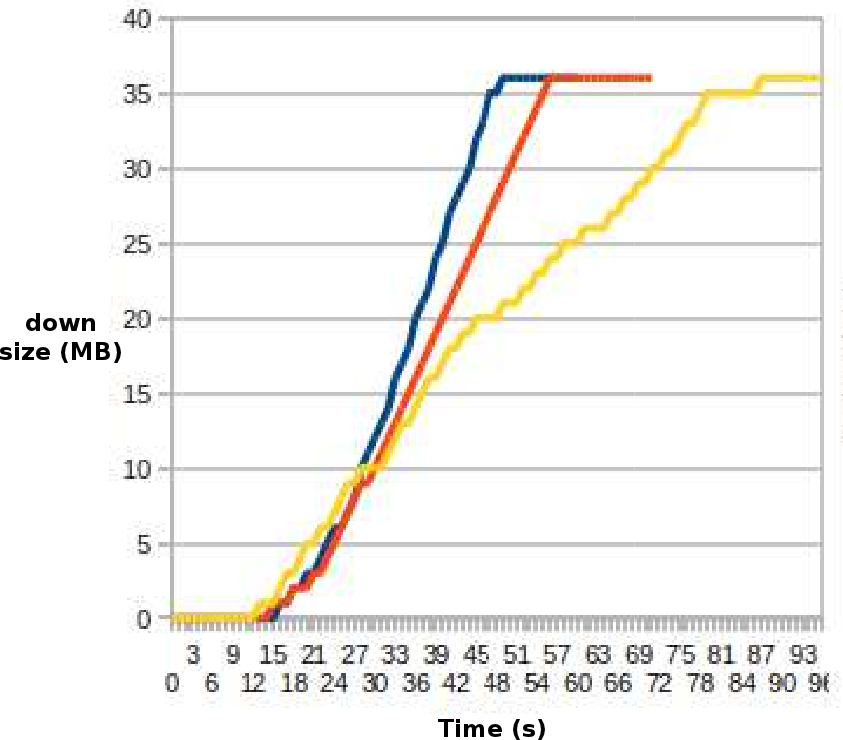
\includegraphics[width=0.35\textwidth]{src/img/multimedia-dist/libtorrent-down-size}
  \label{fig:multimedia-dist:libtorrent-down-size}
  }
  \subfloat[Download Speed Evolution]{
  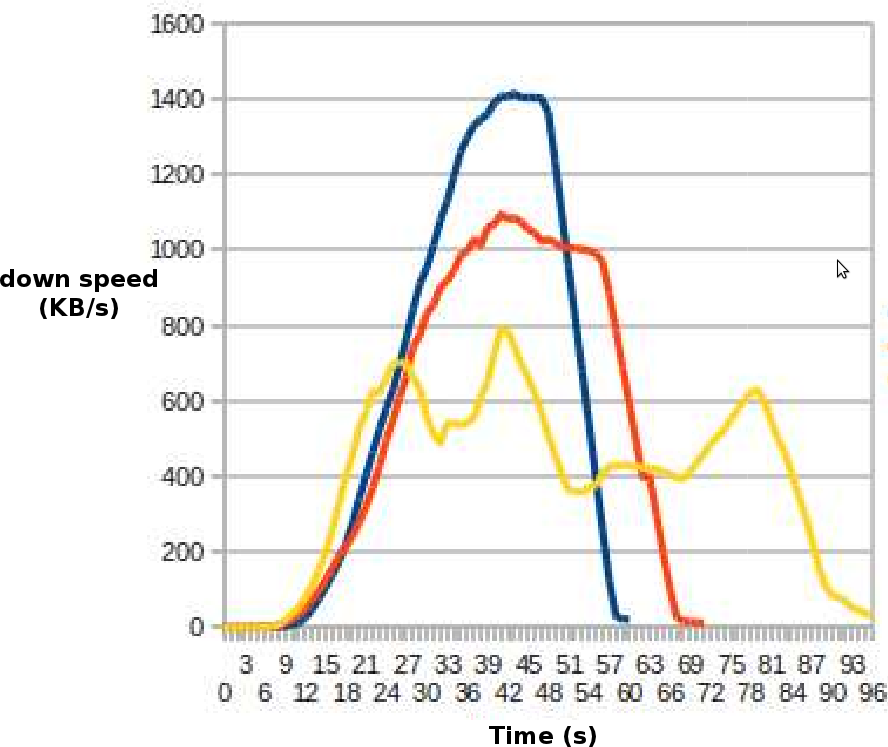
\includegraphics[width=0.35\textwidth]{src/img/multimedia-dist/libtorrent-down-speed}
  \label{fig:multimedia-dist:libtorrent-down-speed}
  }
  \caption{Evolution of Different Piece Selection Policies}
  \label{fig:multimedia-dist:libtorrent-evolution}
\end{figure}

During this experiment, the best algorithm was, as expected, the
\textit{rarest first}. We estimate the \textit{deadline piece} was
outperformed by the \textit{sequential} algorithm, due to the file size being
quite small, a large number of seeders and the implementation overhead of the
former for a relatively small file.

\section{Using Next-Share Technology for P2P Streaming}
\label{sec:multimedia-dist:nextshare}

The P2P-Next project was started in 2008 as an EU FP7 project. It aims at
delivering the next-generation Peer-to-Peer content delivery platform. The
project takes into account the change in the audio video media landscape, with
increased demand for content availability on the Internet and user participation
in generation of content. P2P-Next takes into account existing challenges such
as legal frameworks and business constraints to create a viable solution with
widespread adoption.

Intelligence, resource management, and explicit memory are the foundations for
the P2P-Next content sharing platform called: Next-Share. The Next-Share
system is a self-organizing system with complete decentralisation and hence
lacks any central bottleneck or choke points that may hamper performance,
induce setup cost, or require maintenance. Networking effects ensure that
content, communities, communication, and commerce will flourish with more
participants.

NextShare is a complex architecture integrating features that are common to
BitTorrrent applications but also those integrating streaming content.

NextSharePC runs on PC, supporting Windows, Linux and MacOS X Operating
Systems/distributions. NextSharePC application is formed by two parts:
\begin{itemize}
  \item A back-end server called NextShare Agent (NSSA), which embeds the P2P
  core engine (NextShareCore).
  \item A front-end part in charge of providing the user interface and content
  playback functionalities.
\end{itemize}

The split between front-end and back-end let the P2P engine (NSSA) run in the
background regardless if the front-end interface (GUI) is running or not. This
enables the peer to share content within the NextShare network even if the
user is not in front of the PC and/or is not interacting with NextSharePC.

Initially an improved BitTorrent core aiming for improved performance and
diverse features, the Next-Share core integrated streaming support. This has
been mostly due to Jan David Mol's
work~\cite{give-to-get}~\cite{design-p2p-live} in getting streaming
support in Next-Share. Currently, Next-Share supports both Video-on-Demand
and live streaming. Both stream features are enabled through the use of
mesh-like overlays, regarded as swarm topologies, due to their working on top
of BitTorrent.

VoD support in Next-Share is enabled through the deployment of Give-to-Get, a
novel approach to negotiating piece exchange. Give-to-Get features many
similarities to BitTorrent's own tit-for-tat protocol, but differs in certain
areas which make it more suitable for video-on-demand. Specifically, while in
offline download mode (classical distribution), the tit-for-tat protocol marks
a peer's ``altruism'' by its history, Give-to-Get only checks its recent
history. In VoD, a peer is interested in exchanging information from peers that
can offer him current pieces, in order to sustain video playback; if a peer
has been altruistic with early pieces if of little relevance to the current
peer.

While most implementation use a tree-based or multi-tree based approach for
live streaming, Next-Share's BitTorrent core required a swarm-based approach.
Each peer will connect to a given set of peer and request pieces from those.
Major updates had to be undertaken due to the differences between offline
playback (classical distribution) and live streaming: the size of the file is
unknown, there is no seeder, there are no hashes for integrity checking,
pieces have to be retrieved real time. This required careful updates to the
piece picking component of the BitTorrent engine and the selection of peers in
the neighbor set.

The LivingLab is the mechanism by which Next-Share based application get
tested ``in the while'' i.e. with real users and real environments. In the
P2P-Next project the LivingLabs are located in several partner locations such
as Lancaster (UK), Tromso (Norway), Tampere (Finland), Ljubljana (Slovenia)
and Bucharest (Romania).

The UPB LivingLab consists of several commodity hardware systems kindly
provided by the NCIT cluster. These systems store content used for the
LivingLab and the applications, scripts and services that power it. All
systems are identical both from a hardware perspective and by means of
software applications and content.

The LivingLab site, described in detail in
Section~\ref{subsec:multimedia-dist:evaluation-infrastructure} provides the
interface with the help of which users access content using NextShare
technology. It possess a large number of VoD assets from various events that
are available to be played back using the SwarmPlugin. Assets are HD content
in MP4 and OGG container format. The LivingLab describes useful information to
users and provides a forum where questions may be asked and support may be
requested.

Various experiments have taken place in the UPB LivingLab, the most recent
ones being described in Section~\ref{sec:multimedia-dist:evaluation}. As the
UPB LivingLab is focused on performance management and analysis, experiments
were keen on measuring BitTorrent swarm information and gathering relevant
information.
The current and overall goal of the trials to be deployed and the UPB
LivingLab is comparing Peer-to-Peer streaming performance and functionalities
to classical distribution. We aim to collect relevant internal information
regarding the behavior of the technology both when used for VoD streaming and
for BitTorrent swarm download and use that information for signaling points
that should be taken into account to improve streaming performance, mostly
related to peer download speed.

\section{Evaluation of P2P Streaming Solutions}
\label{sec:multimedia-dist:evaluation}

Within the UPB LivingLab, experiments that involve users, HD content and the
NextShare streaming solutions have and are currently taking place. The goal is
to provide useful information on the functionality of the solution, the user
experience and transfer performance. As the goal of the P2P-Next project
is to built the next-generation Peer-to-Peer content delivery platform, our
aim is to provide useful information regarding key factors that influence its
attractiveness. Questions such as the ones below need to be answered: Would people use this platform instead of
YouTube? Would it outperform classical video streaming? How does it compare to
classical BitTorrent distribution performance?

The UPB LivingLab is the user window to the Next-Share technology. It
provides instructions on using the technology and allows access to the content
and facilities. From a user's point of view,
the LivingLab is the site/portal/frontend allowing the playback of various video
files through the use of P2P technology. In the backend, the LivingLab is
supported by systems in the NCIT cluster that store and serve content in the
form of Video-on-Demand assets.

The NCIT cluster systems are commodity hardware systems that provide content
and seeders. Content is replicated among NCIT cluster systems and is seeded
through automated NextShare technology applications. There are currently nine
systems available. The same content assets are found among multiple systems
such that there would be multiple seeders for each asset. Logging is enabled
at seeder level for subsequent processing. Swarm trackers may reside on a NCIT
system or outside of it; as tracker communication is reduced, its placement is
of little relevance.

User feedback is collected through feedback forms that request information
about user experience, plugins used, issues encountered. Detailed information
about feedback forms is provided in
Section~\ref{subsec:multimedia-dist:evaluation-december-2010}. The feedback
form has been updated from a Google form-based one to one that is fully
integrated into the site. At the same time, during experiment evolutions,
questions were added or were discarded.

A specialized form of user feedback is user log files. During experiments,
both from our side and from WP4 team members, we have requested users to
provide us with logging information for troubleshooting issues. As such, we
have integrated a log upload facility where users can upload basic upload
information provided by NextShare. Log files are typically no greater than
100K, such that there is little overhead or burden in uploading them.

We evaluate streaming performance of NextShare technology through experimental
means. Trials are setup in the LivingLab and use those to collect logging
information and use that for analysis and advice. Providing advice regarding
performance of streaming implementation is the prime concern of our
evaluation.

We use status information such as peer download speed, peer upload
speed, number of connections and extensive information (usually provided
through verbose logging) such as protocol messages, protocol inner workings,
piece picker algorithm (piece selection) to compare and analyze classical
(pure BitTorrent-based data distribution) to video streaming (through
NextShare technology). We aim to distinguish among the various patterns
employed by each type of distribution, measuring variation/penalty in
performance and identify weak and strong spots in each of the approaches.

During December we have undertaken a
medium-sized experiment for evaluating the NextShare technology and user
satisfaction. The LivingLab site was the center of the experiment: it
provided the interface for download the NextShare plugin, linking video files,
publishing the feedback form and providing support through the forum.

A total number of 55 users completed the feedback form. A brief of the
results:
\begin{itemize}
  \item users had problems installing the plugin and most of them were
  unable to properly start the playback;
  \item video playback was deemed mediocre; some may
  be due to the problems in installing the plugin;
  \item the plugin interface was considered to be usable - content playback
  could be easily enabled;
  \item most users used the Firefox version of the Plugin;
  \item users were using high bandwidth connections ($>$ 512KB/s) or fairly
  good ones ($>$ 50KB/s, $<$ 100KB/s);
  \item video freezing and the lack of a seek and volume bar were among the
  most significant remarks.
\end{itemize}

In order to collect information regarding the problems, FTP-based upload form
to allow users to provide us their log files.

The most important issues were problems during the installation and poor video
playback (freezing). One of the main results a similar experiment would need
to provide proper video content (if the problem is from video files), a
properly working version of the NextShare plugin and a seek bar on the
playback interface.

The April 2011 Experiment was focused on testing basic functionality for
comparison between classical distribution versus streaming. The aim is to set
up all pieces required for experimentation, data collection and analysis. In
order to accomplish this data was collected both from classical BitTorrent
clients such as uTorrent, Transmission and streaming functionality. Users were
instructed to use both the NextSharePC plugin and a classical distribution
BitTorrent client in order to provide information required for comparison.

Logging had been enabled at seeder level. Due to the high level of information
only status information such as download speed, upload speed, peer connections
had been collected in log files. A high quantity of data was collected
resulting in 100GB of status log information per seeder in two months time. In
order to match IP information from seeder logs to BitTorrent clients, logging
had also been enabled at tracker level. Tracker log files display global
information regarding swarms and periodic information (typically once every 30
seconds) from announce messages from clients.

Important updates had been implemented since the December experiment, based on
user feedback and updated goals. VLC-based API for playback interaction (such
as a progress bar, volume selection, pause, resume) had been added.

Apart from the VLC-based NextSharePC plugin, the site was added the
Firefox-based plugin using HTML5 technology. Thus, for each VoD assed, there
would be two types of files: MP4+H.264 for the VLC-based plugin and OGG+Theora
for the HTML5-based plugin. Users were provided with links to the other
version of the file. This allowed using NextShare technology on Linux-based
systems.

There were several updates to the site and user interaction, also as part of
user plugin or suggestions from inside the P2P-Next WP4 or WP8 teams. The log
file upload form had been changed from a rather user-unfriendly FTP-based form
to one based on HTTP. The feedback form had also been updated to discard
information that could be retained otherwise (from browser information, for
example – the IP address, operating system, browser, or from BitTorrent client
provided information – average download/upload speed).

42 users had correctly presented their IP addresses. Users had found the
plugin and technology fun to use and provide feedback, both from an average
user's perspective and from a technical user's perspective. Features that have
been praised were:
\begin{itemize}
  \item Fast download speed.
  \item Easy installation.
  \item Good video quality.
\end{itemize}

The issues marked in bold were signaled often. The lack of a volume or
time/progress bar was present in almost all suggestions in the feedback form.

The important issues had been tackled after the trial, some of them being
described in detail in Section~\ref{subsec:multimedia-dist:evaluation-issues}. The most stringent issue deals with
playback problems in the NextShare player for a diversity of video files. This
was due to multiple reasons. One of them of the absence of a bitrate
information in the .torrent/.tstream file; the client was unable to properly
render the video. Another cause was the 

As mentioned, users were requested to use dual clients to provide sample
information from classical BitTorrent distribution clients and from the
NextSharePC plugin as a representative of P2P streaming solutions. Download
and upload rate for the NextSharePC is limited to 1MB/s for performance
consideration such that preliminary results have little relevance other than
providing sample information and testing the existing infrastructure.

Sample results were:

\begin{itemize}
  \item ``classical'' clients used (no recommendation was given to users)
  were: uTorrent (16), Transmission (9) and BitTorrent mainline (2)
  \item NextSharePC download speed varied between 300KB/s and 800KB/s
  \item Transmission download speed: 500KB/s-1500KB/s
  \item uTorrent download speed: 1000KB/s-4000KB/s
\end{itemize}

Figure~\ref{fig:multimedia-dist:ds-evolution-full} represents the download
speed by client types during a wider window of the April 2011 trial.
Figure~\ref{fig:multimedia-dist:ds-evolution-day} uses a smaller window
centered around a time interval that provided a high number of client
connections (between 8:00PM and 11:00PM on April 13, 2011). Each client type
uses a specific color in the figure. As noticed, the NextSharePC client is
limited to 1MB/s, while Transmission and uTorrent usually perform better. As
users were requested to use NextSharePC and another client, the NextSharePC
client is responsible for a large chunk of the plot.

\begin{figure}
  \centering
  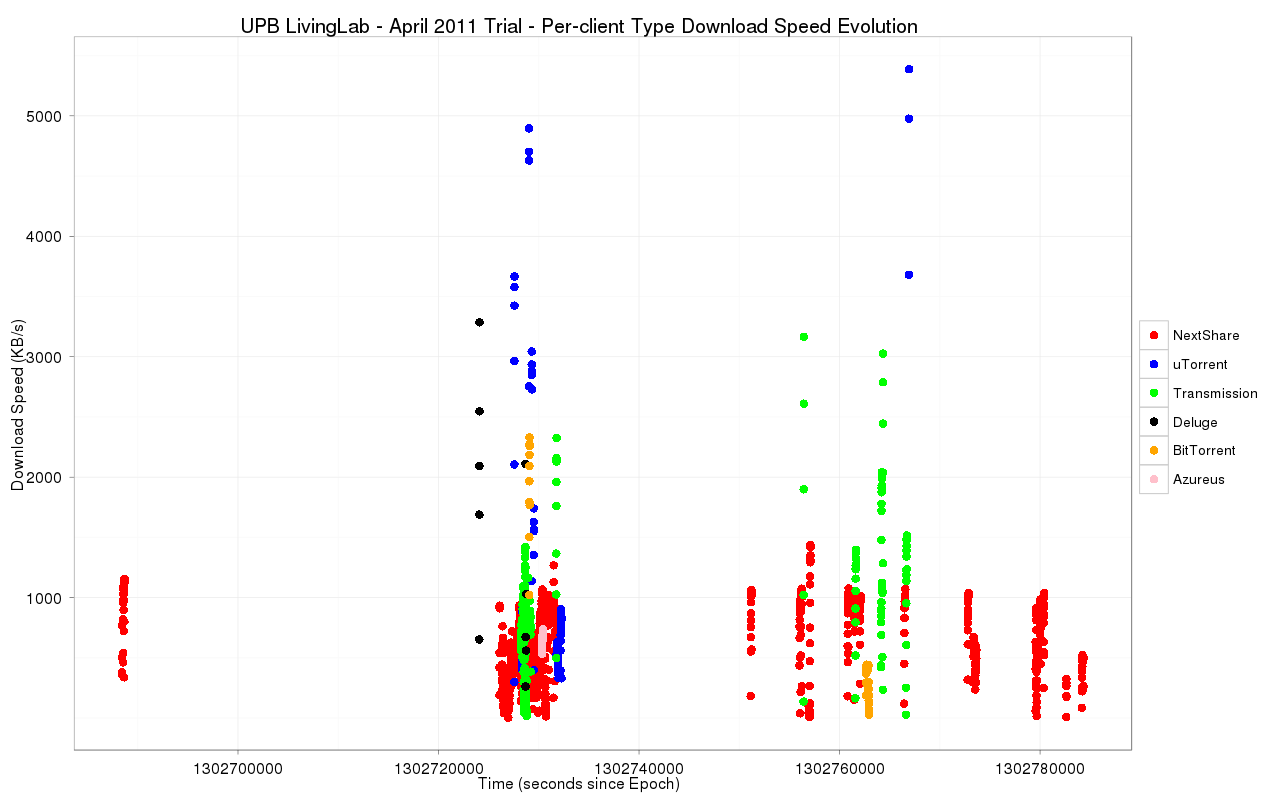
\includegraphics[width=0.6\textwidth]{src/img/multimedia-dist/ds-evolution-full}
  \caption{April Trial -- Download Speed Evolution by Client Type}
  \label{fig:multimedia-dist:ds-evolution-full}
\end{figure}

\begin{figure}
  \centering
  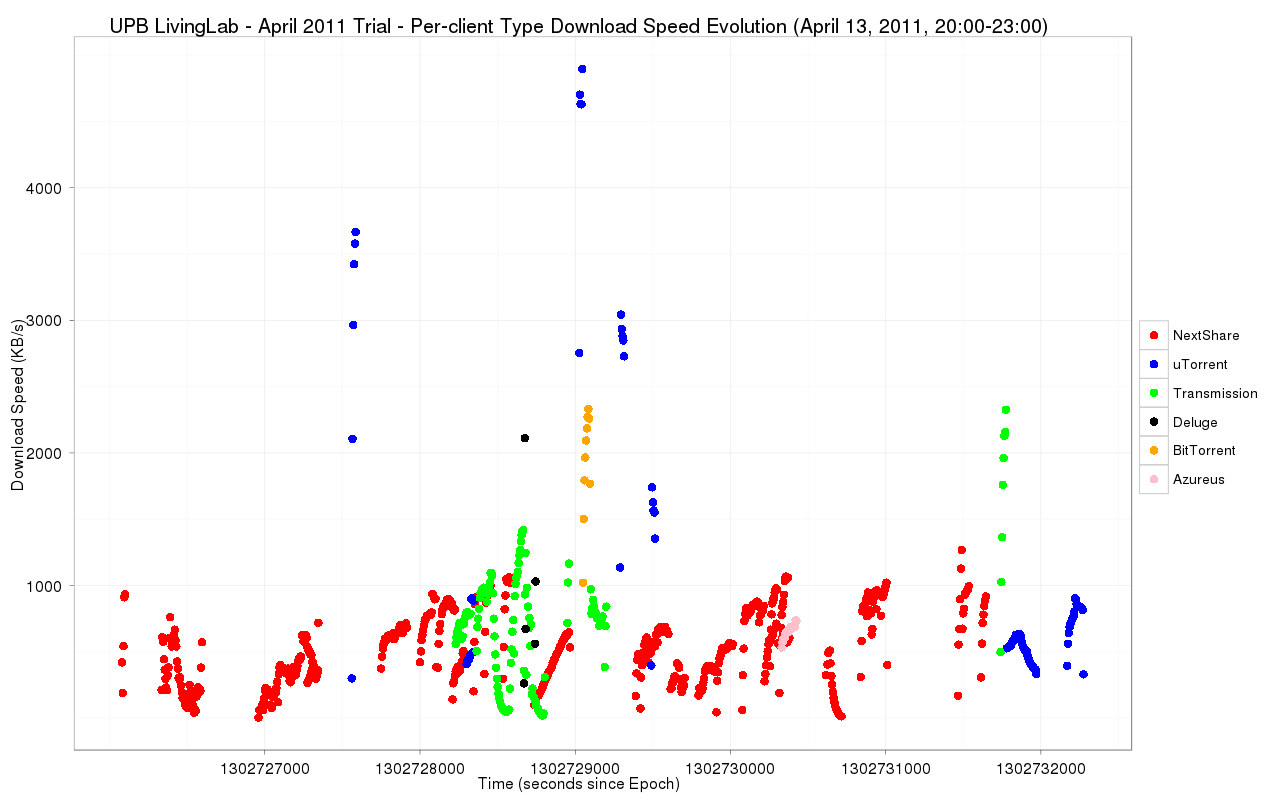
\includegraphics[width=0.6\textwidth]{src/img/multimedia-dist/ds-evolution-day}
  \caption{April Trial -- Download Speed Evolution by Client Type
  (8:00PM-11:PM, April 13, 2011)}
  \label{fig:multimedia-dist:ds-evolution-day}
\end{figure}
